% gc-01-Functions.tex

\documentclass[xcolor=dvipsnames]{beamer}
\usepackage{teachbeamer}

\title{Functions}
\subtitle{MATH {\CourseNumber}, BCIT}

\author{\CourseName}

\date{January 5, 2018}

% \begin{figure}[h]
% 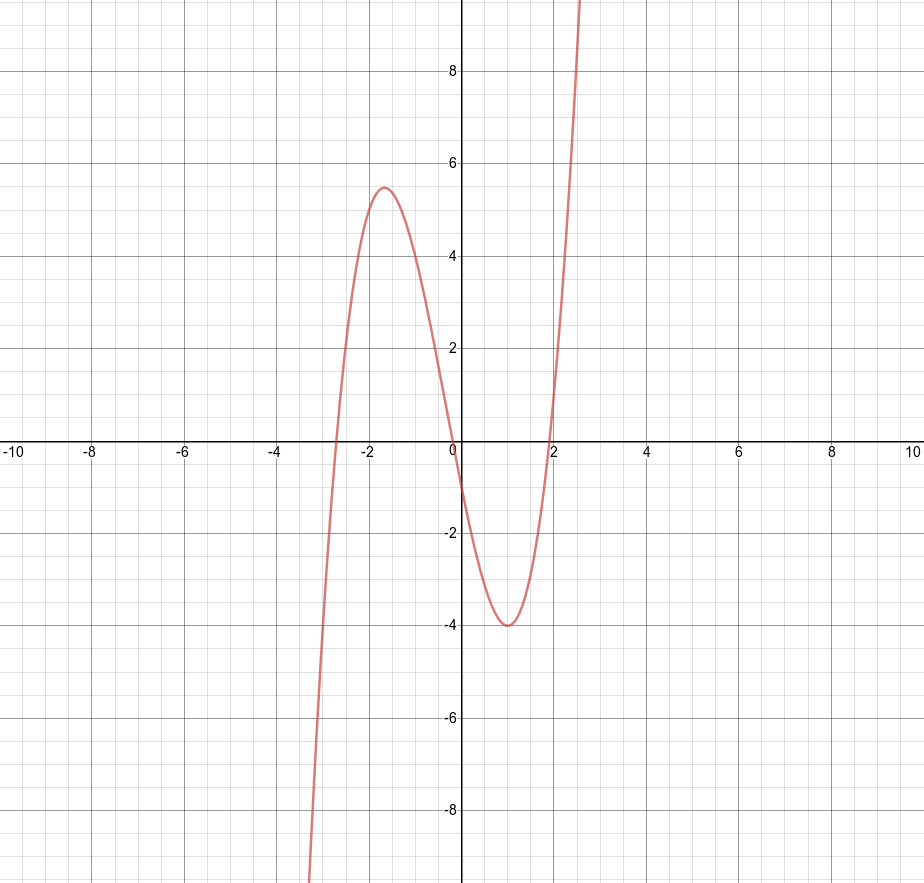
\includegraphics[scale=.3]{./extrema1.png}
% \end{figure}

\begin{document}

\begin{frame}
  \titlepage
\end{frame}

\begin{frame}
  \frametitle{The Exponential Function: Graph}
Let's have a look at the graph for the exponential function.
  \begin{figure}[h]
    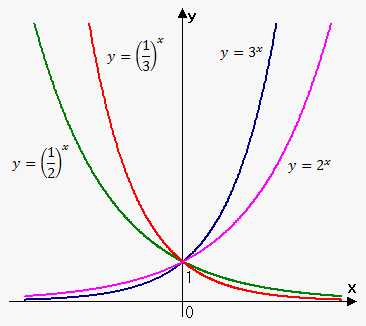
\includegraphics[scale=.6]{./1_2_exponential_function.png}
  \end{figure}
\end{frame}

\begin{frame}
  \frametitle{The Exponential Function: Properties}
  Here are some properties for the following exponential function
  ($a>0$),
\begin{equation}
  \label{eq:muwauzie}
  f(x)=a^{x}
\end{equation}
\end{frame}

\begin{frame}
  \frametitle{The Exponential Function: Properties}
\begin{itemize}
\item<1-> if $a=1$ then the exponential function is the constant function $f(x)=1$
\item<2-> $f(0)=1$ and $f(1)=a$
\item<3-> the domain of $f$ is the real numbers, the range of $f$ is
  all positive real numbers, and $f$ is injective (one-to-one)
\item<4-> if $a>1$ then $f(x)$ tends to $0$ as $x\rightarrow -\infty$, and
  $f(x)$ goes very fast to $+\infty$ as $x\rightarrow \infty$
\item<5-> if $a<1$ then $f(x)$ tends to $0$ as $x\rightarrow \infty$, and
  $f(x)$ goes very fast to $+\infty$ as $x\rightarrow -\infty$
\item<6-> how fast the graph rises to $+\infty$ on the left or the
  right depends on how large $a$ is (if $a>1$) or how small
  $a$ is (if $a<1$). The closer $a$ is to $1$, the flatter the graph.
  `Flat,' of course, is a relative term here: no matter how close $a$
  is to $1$, the function graph will still rise faster than any polynomial.
\end{itemize}
\end{frame}

\begin{frame}
  \frametitle{Functions}
Here are a few definitions,
\begin{description}
\item[function] A function assigns a unique element of a set to each
  element of another (not necessarily distinct) set.
\item[domain] The domain is the set of elements to which the function
  assigns a unique element.
\item[codomain] The codomain is the set from which the function picks
  out elements to assign.
\item[range] The range is the subset of the codomain whose elements
  the function assigns to an element in the domain.
\item[injective] A function is injective if it does not assign the
  same element of the codomain to two distinct elements in the domain.
\item[surjective] A function is surjective if there are no elements in
  the codomain which are not assigned to an element in the domain.
\end{description}
\end{frame}

\begin{frame}
  \frametitle{Examples}
What are possible domains and ranges for the following functions? Are
the functions injective or surjective, given a particular domain and
codomain?
\begin{equation}
  \label{eq:rebiejie}
  f(x)=2x+3
\end{equation}
\begin{equation}
  \label{eq:ebaivuim}
  f(x)=x^{2}-1
\end{equation}
\begin{equation}
  \label{eq:ichievae}
  f(x)=\sqrt{x+4}
\end{equation}
\begin{equation}
  \label{eq:ejawache}
  f(x)=\frac{1}{x+7}
\end{equation}
\begin{equation}
  \label{eq:tohjuogi}
  f(x)=10^{2x}
\end{equation}
\end{frame}

\begin{frame}
  \frametitle{Inverse Functions}
If a function $f$ from a domain to a codomain is injective, then there
is a function $f^{-1}$ from the range of $f$ to its domain which has
the following property,
\begin{equation}
  \label{eq:noexiedi}
  f^{-1}(y)=x\mbox{ if and only if }f(x)=y
\end{equation}
We call $f^{-1}$ the \alert{inverse function} of $f$. Let, for
example,
\begin{equation}
  \label{eq:iengaihu}
  f(x)=4x-3
\end{equation}
Replace $f(x)$ by $y$ for the equation $y=4x-3$ and manipulate the
equation to isolate $x$. Then replace $x$ by $f^{-1}(y)$ for the
inverse function
\begin{equation}
  \label{eq:eimoofie}
  f^{-1}(y)=\frac{y+3}{4}
\end{equation}
\end{frame}

\begin{frame}
  \frametitle{Defining Logarithms}
Let $f$ be an exponential function with a base $a>1$,
\begin{equation}
  \label{eq:ohzuiwah}
  f(x)=a^{x}
\end{equation}
Considering the function graph of this exponential function, it is
apparent that $f$ is an injective and surjective function for the
domain $\mathbb{R}$ and the codomain $\mathbb{R}^{+}$.
$\mathbb{R}^{+}$ is the set of all positive real numbers. There is
therefore an inverse function from $\mathbb{R}^{+}$ to the real
numbers, which we shall call $\log_{a}$,
\begin{equation}
  \label{eq:cievucha}
  \log_{a}(y)=x\mbox{ if and only if }a^{x}=y
\end{equation}
\end{frame}

\begin{frame}
  \frametitle{Functions}
A \alert{function} is a rule that assigns to each element in a set $A$ one and
only one element in a set $B$.

\medskip

\emph{Exercise:} Find the maximum domain and range of the following
functions on the real number line:
\begin{equation}
  \label{eq:sijoomai}
  f(x)=\sqrt{x-1}
\end{equation}
\begin{equation}
  \label{eq:vooghahk}
  f(x)=\frac{1}{x^{2}-4}
\end{equation}
\begin{equation}
  \label{eq:zaekohxi}
  f(x)=x^{2}+3
\end{equation}
\end{frame}

\begin{frame}
  \frametitle{Function Graphs}
The \alert{graph of a function} $f$ is the set of all points $(x,y)$
in the $xy$-plane such that $x$ is in the domain of $f$ and $y=f(x)$.
  \begin{figure}[h]
    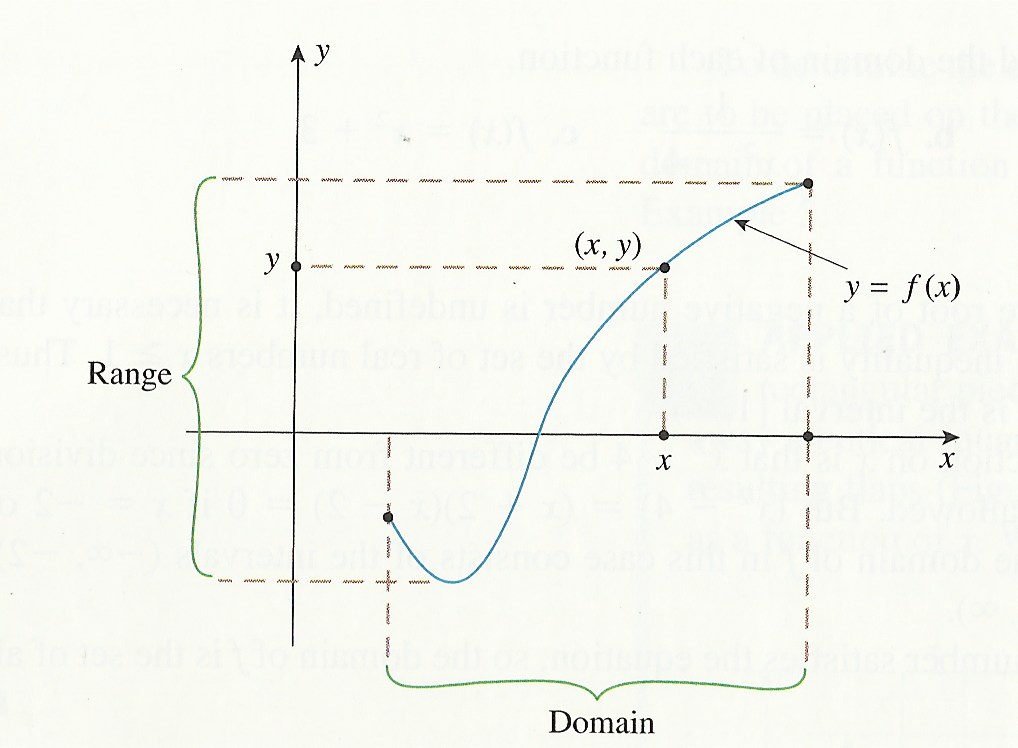
\includegraphics[scale=1]{./fgraph-02.png}
  \end{figure}
\end{frame}

\begin{frame}
  \frametitle{Vertical Line Test}
Every function $f$ on a subset of the real numbers has a function
graph, but not all graphs correspond to a function. Consider the graph
$y^{2}=x$. A curve in the $xy$-plane is the graph of a function
$y=f(x)$ if and only if each vertical line intersects it in at most
one point.
  \begin{figure}[h]
    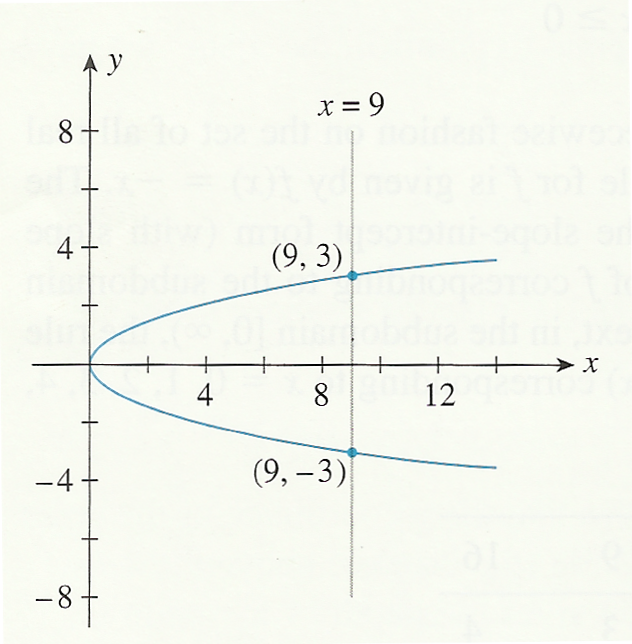
\includegraphics[scale=1]{./fgraph-03.png}
  \end{figure}
\end{frame}

\begin{frame}
  \frametitle{Vertical Line Test Exercise}
In the next four slides, determine which graphs correspond to a function.
\end{frame}

\begin{frame}
  \frametitle{Vertical Line Test Exercise I}
  \begin{figure}[h]
    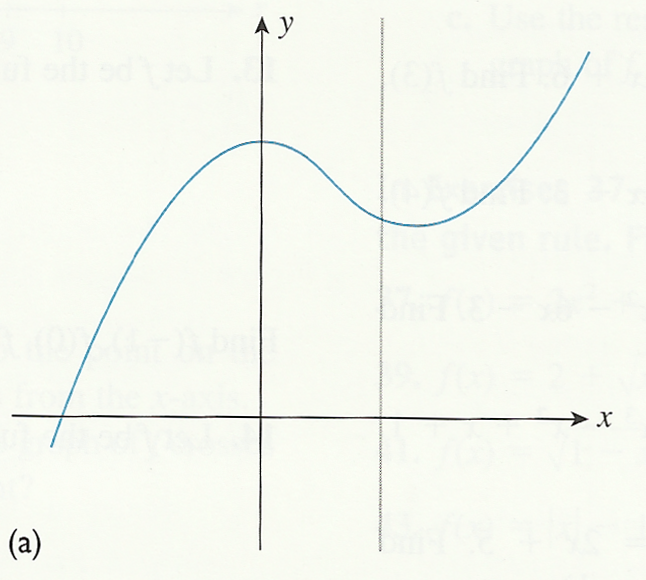
\includegraphics[scale=1]{./vertical-01.png}
  \end{figure}
\end{frame}

\begin{frame}
  \frametitle{Vertical Line Test Exercise II}
  \begin{figure}[h]
    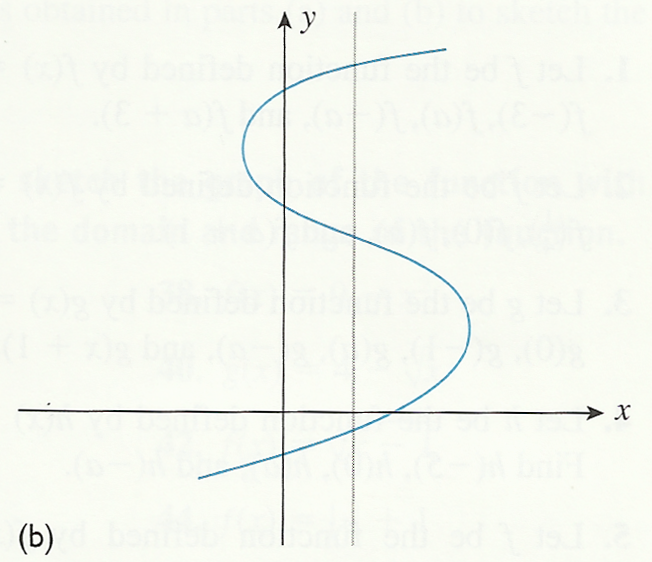
\includegraphics[scale=1]{./vertical-02.png}
  \end{figure}
\end{frame}

\begin{frame}
  \frametitle{Vertical Line Test Exercise III}
  \begin{figure}[h]
    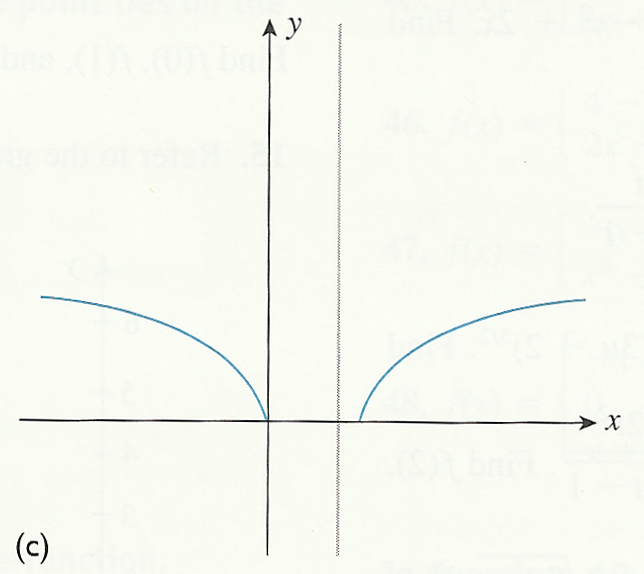
\includegraphics[scale=1]{./vertical-03.png}
  \end{figure}
\end{frame}

\begin{frame}
  \frametitle{Vertical Line Test Exercise IV}
  \begin{figure}[h]
    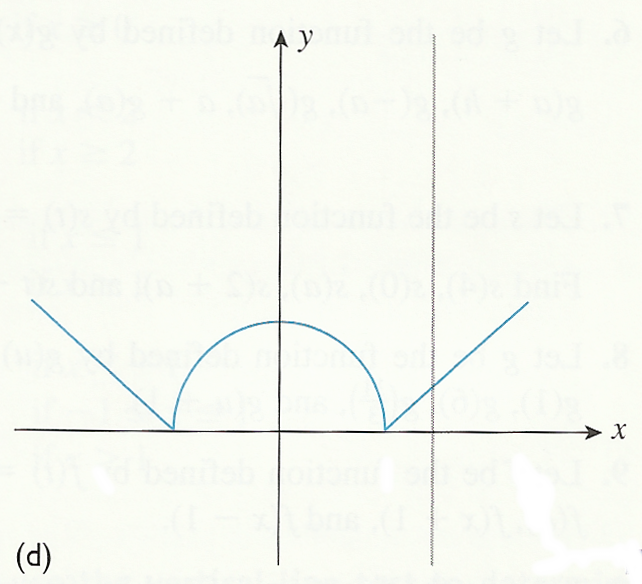
\includegraphics[scale=1]{./vertical-04.png}
  \end{figure}
\end{frame}

\begin{frame}
  \frametitle{Function Algebra}
Let $f$ and $g$ be functions with domain $A$ and $B$, respectively.
Then the \alert{sum} $f+g$, \alert{difference} $f-g$, and
\alert{product} $fg$ of $f$ and $g$ are functions with domain
$A\cap{}B$ (the intersection of $A$ and $B$) and rule given by
\begin{equation}
  \label{eq:maichong}
  (f+g)(x)=f(x)+g(x)
\end{equation}
\begin{equation}
  \label{eq:pieshouz}
  (f-g)(x)=f(x)-g(x)
\end{equation}
\begin{equation}
  \label{eq:queebeih}
  (fg)(x)=f(x)\cdot{}g(x)
\end{equation}
The \alert{quotient} $f/g$ of $f$ and $g$ has domain $A\cap{}B$
excluding all points $x$ such that $g(x)=0$ and rule given by
\begin{equation}
  \label{eq:thaochao}
  \left(\frac{f}{g}\right)(x)=\frac{f(x)}{g(x)}
\end{equation}
\end{frame}

\begin{frame}
  \frametitle{Function Composition}
Let $f$ and $g$ be functions. Then the \alert{composition} of $g$ and $f$ is
the function $g\circ{}f$ defined by
\begin{equation}
  \label{eq:aphiepae}
  (g\circ{}f)(x)=g(f(x))
\end{equation}
The domain of $g\circ{}f$ is the set of all $x$ in the domain of $f$
such that $f(x)$ lies in the domain of $g$.

\medskip

Consider the following two functions, $f(x)=\sqrt{x}$ and
  $g(y)=y-2$. What are the maximal domains in the real numbers of
  $f\circ{}g$ and $g\circ{}f$?
\end{frame}

\begin{frame}
  \frametitle{End of Lesson}
Next Lesson: Limits.
\end{frame}

\end{document}
